%Schriftgröße, Dokumentformat, Dokumenttyp
\documentclass[11pt,a4paper]{article}
%Einstellungen der Seitenränder
\usepackage[left=3cm,right=4cm,top=2cm,bottom=2cm,includeheadfoot]{geometry}
%neue Rechtschreibung und Formelsatz
\usepackage[utf8]{inputenc}
\usepackage[english]{babel}
\usepackage[T1]{fontenc}
\usepackage{textcomp}
\usepackage{amsmath,amssymb,amsthm}
%Graphiken
\usepackage{graphicx}
\usepackage{float}
%Zeilenabstand
\usepackage{setspace}\onehalfspacing
%Aufzählungen
\usepackage{paralist}
%Abkürzungen
\usepackage{acronym}
%Tabelle
\usepackage{multirow}
%Kopf- und Fußzeile
\usepackage{fancyhdr}
%Fußnotenkram
\usepackage{footnote}
\usepackage{hyperref}
\usepackage[hang]{footmisc}
\usepackage{graphics}
\usepackage{glossaries}
\setlength{\footnotesep}{0.25 cm}


\begin{document}
% Keine Seitenzahlen im Vorspann
\pagestyle{empty}
	
%%%%%%%%%%%%%%%%%%%%%%% Titelblatt der Arbeit %%%%%%%%%%%%%%%%%%%%%%%
\begin{titlepage}				
	\begin{center}
Professorship for XXX\\
Institute of XXX\\
Faculty of Business, Economics and Social Sciences\\
Kiel University \\
		\vspace{5cm}
		
		\LARGE{ \bf{Density Forecasts of the S\&P using Markov-Switching Models}}
		\vspace{2cm}
		
		\large{\bf{Seminar paper}}\\
		Submission Date: XX.XX.XXXX
		\vspace{1.5cm}

\begin{flushleft}
\vfill
	Author: Adrian Beer
	Subject:\\
	Semester:3
	Module: Seminar in Econometrics
	Stu-Email-Adress:\\
	Matriculation number:\\
	\vspace{1cm}
	First Assessor:\\
	Second Assessor:
\end{flushleft}	
		
				
	\end{center}

\end{titlepage}


%%%%%%%%%%%%%%%%%%%%%%% Inhaltsverzeichnis %%%%%%%%%%%%%%%%%%%%%%%


\newpage
	\tableofcontents
	\newpage


% Kopf- und Fußzeile definieren 
\pagestyle{fancy}					
\fancyhf{}								
%Kopfzeile rechts bzw. außen			
\fancyhead[R]{}							 
%Linie oben								 
\renewcommand{\headrulewidth}{0pt}	 
%Fußzeile mittig					 
\fancyfoot[R]{\thepage}				 
%Linie unten										
\renewcommand{\footrulewidth}{0pt}	 
%Seitenzahlen ab hier						 
\pagenumbering {Roman} 
\setcounter{page}{1}



%%%%%%%%%%%%%%%%%%%%%%%%%%%%% List of Figures %%%%%%%%%%%%%%%%%%%%%%%%%%%%%%%%%
\addcontentsline{toc}{section}{Figure directory}
\listoffigures


\newpage
%%%%%%%%%%%%%%%%%%%%%%%%%%%%% List of Tables %%%%%%%%%%%%%%%%%%%%%%%%%%%%%%%%%
\addcontentsline{toc}{section}{Table directory}
\listoftables
\newpage

%%%%%%%%%%%%%%%%%%%%%%%%%%%%% List of Acronyms %%%%%%%%%%%%%%%%%%%%%%%%%%%%%%%
\section*{List of Acronyms} %Bitte alphabetisch ordnen!
\addcontentsline{toc}{section}{Abbreviation directory}
\rule[0pt]{0mm}{10pt}
\noindent Include an abbreviation directory if you use more than three uncommon abbreviations.\\

\begin{tabular}{l l l}


	% B
	BLL && Bayesian Local Likelihood\\
	BR&&Bounded Rationality\\
	% D
	DSGE&&Dynamic Stochastic General Equilibrium\\


\end{tabular}

\newpage

%%%%%%%%%%%%%%%%%%%%%%%%%%%%% List of Symbols %%%%%%%%%%%%%%%%%%%%%%%%%%%%%%%
\section*{List of Symbols} 
\addcontentsline{toc}{section}{Symbol directory}
\noindent Include a symbol directory if you use more than three uncommon abbreviations.
	\begin{tabular}{l l}
		\textbf{} & \\
		$\pi$ & rate of inflation\\
		$i$ & nominal interest rate \\
		$r$ & real interest rate \\
		$M$ & money stock \\


	\end{tabular}\\ \vspace{1cm}

								
		
		


\newpage


% Kopf- und Fußzeile definieren %%
\pagestyle{fancy}						
\fancyhf{}								
%Kopfzeile rechts bzw. außen			
\fancyhead[R]{}							 
%Linie oben								 
\renewcommand{\headrulewidth}{0pt}	 
%Fußzeile mittig					 
\fancyfoot[R]{\thepage}				 
%Linie unten										
\renewcommand{\footrulewidth}{0pt}	 
%Seitenzahlen ab hier						 
\pagenumbering {arabic}
\onehalfspacing	
\section{Introduction}
Markov chain processes can be useful for identifying regimes in the past as well as estimating the current regime. %% why is this important
If the Markov model describes the data generating process well, it can also be used to simulate synthetic time series and potential future paths. %% why is this important

We test 3 models: 
1. A naive forecast, i.e. we estimate a model/ density which assumes i.i.d. observations. 
2. A markov-switching model without indicators
3. A markov-switching model with indicators

\section{Background}

There are two main ways to learn the parameters of a HMM model: Expectation-Maximization Algorithms (EM) such as Baum-Welch. And Markov Chain Monte Carlo methods (MCMC) such as the Metropolis-Hastings or Gibbs Sampling algorithm.

The EM Algorithm makes use of the forward-backward algorithm.

Given a HMM model we can deduce estimates of the hidden state via the Viterbi algorithm.

\section{HMM with time-varying transition probabilities}
Our goal is to maximize the incomplete data log-likelihood $\log f(y \mid X ; \theta)=\log \sum_{s_{1}=1}^{2} \sum_{s_{2}=1}^{2} \ldots \sum_{s_{T}=1}^{2} f(y, s \mid X ; \theta)$ which is not feasible to compute (complexity). \\
Hence we maximize the expected value of the complete data log-likelihood $\log f(y, s \mid X ; \theta)$. Let $Y_t$ be the natural filtration of $Y$ and $\mathbb{X}_t$.
\section{First chapter of main text}

Divide your text into chapters (1; 2; 3; ...), sections (1.1; 1.2; 1.3; ...) and subsections (2.1.1; 2.1.2; 2.1.3; ...). A bullet point 2.1.1 is nonsensical unless a bullet point 2.1.2 follows. Give all chapters, sections, and subsections expressive headings.
\newpage

\subsection{First section of first chapter of main text}
This section is nonsensical unless a section 2.2 follows.

\subsubsection{First subsection}
This subsection is nonsensical unless a section 2.1.2 follows. You may include a table in this section. Label the table and indicate the source including the page number like you would in the continuous text. The contents of the table below are taken from the highly cited Smets \& Wouters (2007: 597).
\begin{table}[H]
	\centering
	\resizebox{\textwidth}{!}{%
		\begin{tabular}{cccccccccccccc}
			\hline \hline
			&&&&&&&&&&&&&\\
			&	Base& & $\xi_p=0.1$ & &$\xi_w=0.1$ & & $\iota_p\approx0.0$&& $\iota_w\approx0.0$ &&$\phi=0.1$ && $\lambda=0.1$ \\
			\cline{2-2} \cline{4-4} \cline{6-6} \cline{8-8} \cline{10-10} \cline{12-12} \cline{14-14} 
			\textit{Est. Mode}&&&&&&&&&&&&&\\
			$\varphi$ & 5.48&& 4.41 && 2.78 && 5.45 &&5.62 && 0.1 && 1.26\\
			$\sigma_c$& 1.39 && 1.31 && 1.80 && 1.43 && 1.42 && 2.78&& 2.90\\
			$\sigma_l$&1.92&&1.48&&0.25&&1.91&&1.91&&5.24&&1.21\\
			$\lambda$&0.71 && 0.70 && 0.34 && 0.70&& 0.71&& 0.12 && 0.10\\
			$\xi_w$&0.73&& 0.55&&0.10&&0.75&&0.75&&0.89&&0.73\\
			$\xi_p$&0.65&&0.10&&0.48&&0.66&&0.69&&0.86&&0.62\\
			$\iota_p$&0.22&&0.84&&0.24&&0.01&&0.24&&0.08&&0.21\\
			$\iota_w$&0.59&&0.71&&0.68&&0.61&&0.01&&0.39&&0.61\\
			$r_\pi$&2.03&&2.15&&2.15&&2.01&&2.01&&2.03&&2.24\\
			$r_y$&0.08&&0.08&&0.08&&0.08&&0.09&&0.23&&0.12\\
			$r_{\Delta y}$&0.22&&0.21&&0.25&&0.22&&0.22&&0.30&&0.29\\
			&&&&&&&&&&&&&\\
			\textit{Marg. LH} & && && && && && &&\\
			&-923&&-975&&-973&&-918&&-927&&-1084&&-959\\
			&&&&&&&&&&&&&\\
			\hline \hline
	\end{tabular}}
	\caption[Example table (short description)]{An example table. Describe it shortly. Source: Smets \& Wouters (2007): 597.}
\end{table}
\newpage
 \subsubsection{Second Subsection}
You may want to include a figure here. Label the figure and include the source. You may also want to include a second figure that you created yourself.
 \begin{figure}[H]
 	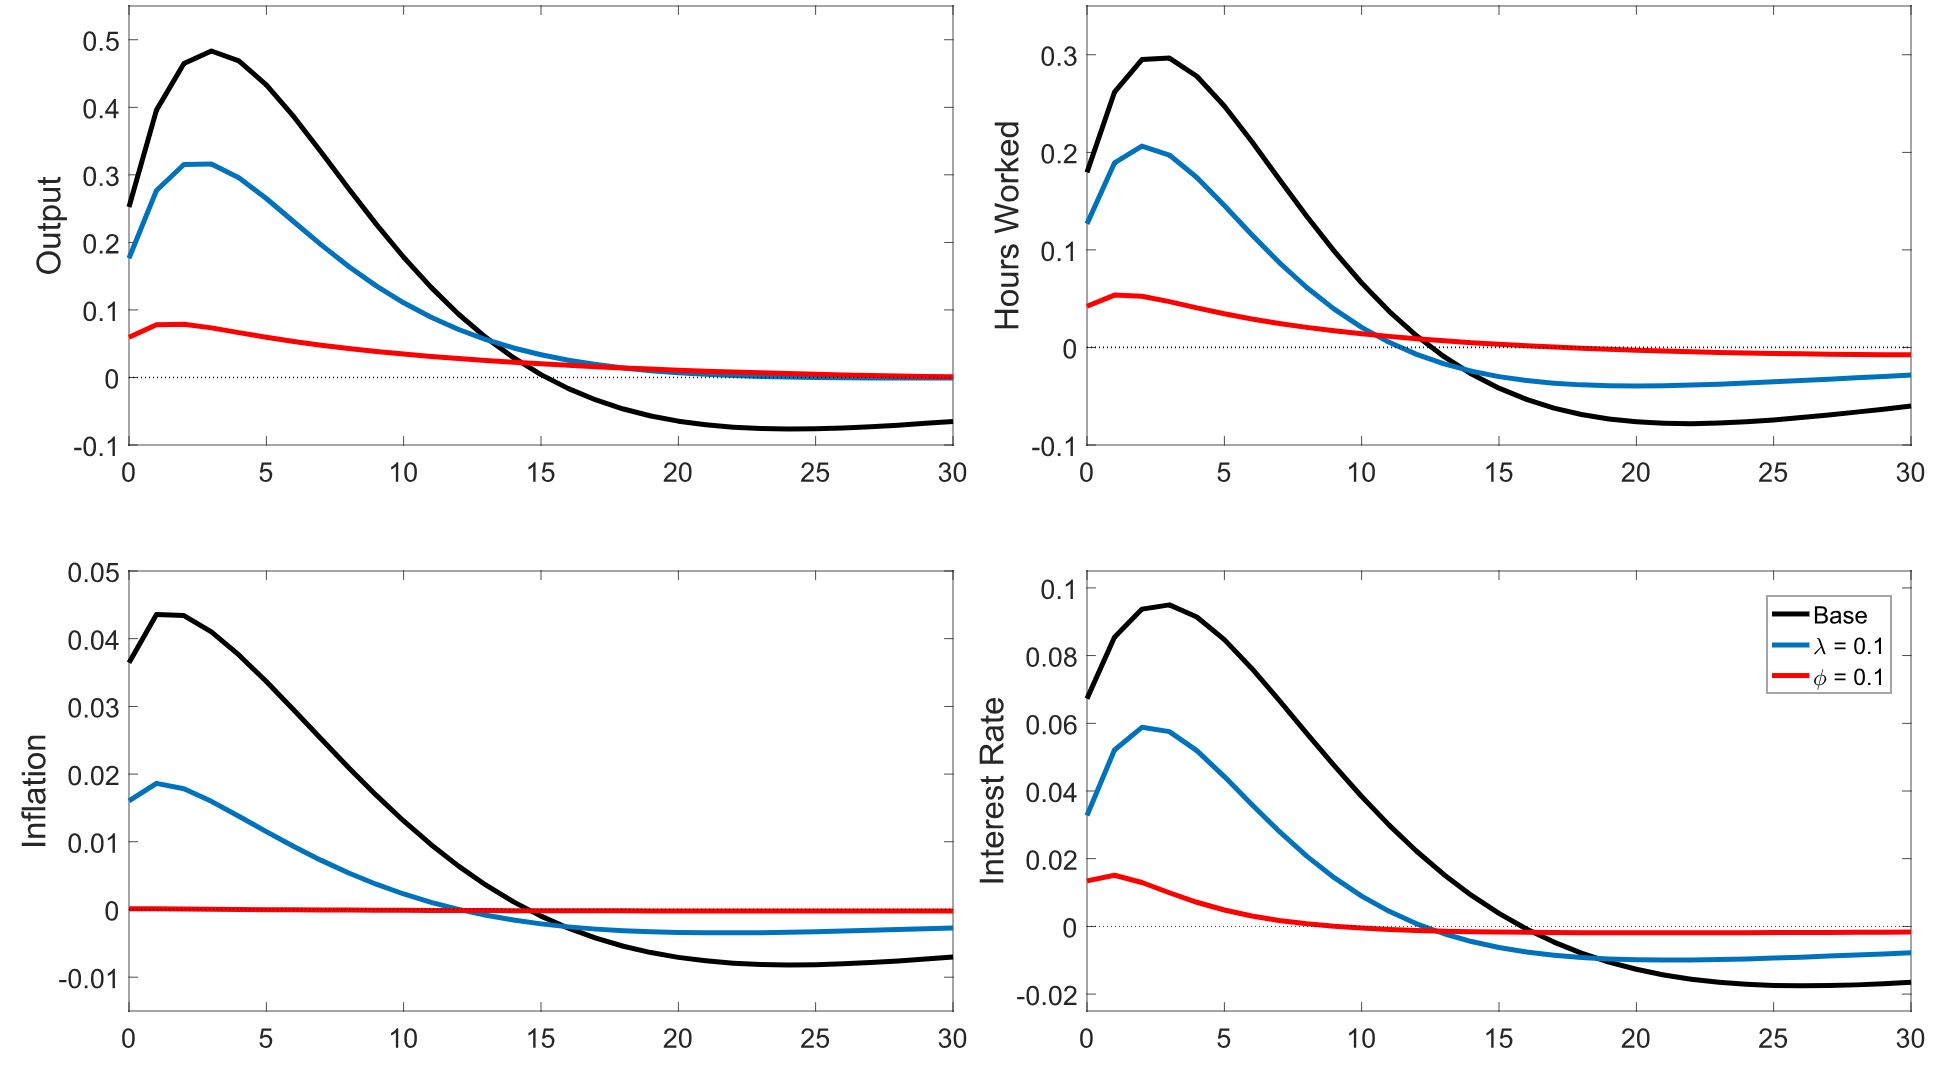
\includegraphics[width=\textwidth]{example_figure}
 	\caption[Short description]{IRFs. SW baseline model with standard calibration (black line, appendix table 8), with low habits in consumption (blue line, table 1) and with low capital adjustment cost (blue line, table 1). Source: Own simulation.}
 \end{figure}
\newpage
\subsection{Second section of first chapter of main text}
This section follows section 2.1 with its subsections. Make it clear how sec-tions and chapters in your work link together. Some introductory and guiding sentences may help the reader and yourself not to lose track of the line of reasoning.

\newpage

\section{Second chapter of main text}

The main text can consist of several chapters, sections and subsections.\\
Use paragraphs to divide the body text within the (sub) chapters into mean-ingful sections. Paragraphs that are longer than one page are usually too long. The reader will not remember upon reaching the end of the paragraph what the main message was. On the other hand, a paragraph that consists of only one sentence is likely too short.\\
If you include illustrations, tables and / or equations in the text, explain them to the reader and describe the results in the text. When using symbols in the text, include their meaning (for example, the money stock M).


\newpage



\section{Conclusion}
End your work with a chapter in which you summarize your findings, formulate some theses, or point out unsolved problems.\\
Before submitting your work, check the following (non-exhaustive) checklist to see if you have met the basic requirements of a well-crafted seminar pa-per, bachelor or master thesis.
\begin{itemize}
	\item Does the text still contain spelling or punctuation errors?
	\item Do you use a fluent and understandable way of expression?
	\item Are words, passages or entire pages missing?
	\item Does the table of contents (and other directories) match the structure of the text and page numbers?
	\item Is the bibliography complete? (Delete bibliography entries that you do not cite!)
	\item Are all references to literature, figures and appendix correct? Did you forget any references?
	\item Is the layout (headings, text formatting, etc.) clear and consistent?
	\item Did you include all necessary components of a scientific paper?
	\item Did you correctly number figures, tables, footnotes, equation?
	
\end{itemize}
\newpage



% Kopf- und Fußzeile definieren 
\pagestyle{fancy}						
\fancyhf{}								
%Kopfzeile rechts bzw. außen			
\fancyhead[R]{}							 
%Linie oben								 
\renewcommand{\headrulewidth}{0pt}	 
%Fußzeile mittig					 
\fancyfoot[R]{\thepage}				 
%Linie unten										
\renewcommand{\footrulewidth}{0pt}	 
%Seitenzahlen ab hier						 
\pagenumbering {Roman} 
\setcounter{page}{5}
\newpage\clearpage

\newpage
\addcontentsline{toc}{section}{Bibliography}
\section*{Bibliography}
In the bibliography, you list all the sources that you use and therefore cite in the text (sources that you have read but not cited should not be listed). Sort the entries in the bibliography, listed according to a consistent style, alphabetically by last name.
\begin{itemize}
	\item[] Adolfson, M.; Las\'een, S.; Lind\'e, J. (2007): Bayesian Estimation of an Open Economy DSGE Model with Incomplete Pass-Through, \textit{Journal of International Economics} 72 (2): 481-511.
 \item[] Christiano, L.; Eichenbaum, M.; Evans, C. (2005): Nominal Rigidities and the Dynamic Effects of a Shock to Monetary Policy, \textit{Journal of Political Economy} 113 (1): 1-45.
 \item[] Hommes, C.; Makarewicz, T.; Massaro, D.; Smits, T. (2017): Genetic Algorithm Learning in a New Keynesian Macroeconomic Setup, \textit{Journal of Evolutionary Economics} 27: 1133-1155.
	\item[] Smets, F.; Wouters, R. (2007): Shocks and Frictions in US Business Cycles: A Bayesian DSGE Approach, \textit{The American Economic Review} 97: 
	\item[] Wieland, V.; Wolters, M. (2012): Forecasting and Policy Making, \textit{IMFS Working Paper Series} No. 62.
\end{itemize}


\newpage

\addcontentsline{toc}{section}{Appendix}
\begin{appendix}
	The appendix contains tables, data, questionnaires, proofs, derivations, etc., which you consider merely additional information and negatively affect the reading flow in the main text. Do not use the appendix for outsourcing text that does not fit into the main text due to page restrictions. Only include an appendix when needed.
	\section{Equality of 1 and 2}
	\label{proof:1equal2}
	\begin{align}
	x^2 &= x^2 \\
	x^2 - x^2 &= x^2 - x^2 \\
	x^2 - x^2 &= x^2 - x^2 + x^2 - x^2	\\
	x\cdot\left(x-x\right) &= \left(x+x\right)\cdot\left(x-x\right)	\\
	x &= \left(x+x\right)	\\
	1 &= 2	\hspace{1cm} q.e.d.
	\end{align}
\section{Latex examples}
\begin{table}
	\centering\rotatebox{90}{%
		\resizebox{\textheight}{!}{%
			\begin{tabular}{lccccccccccccccccccc}
				\hline \hline
				&&&&&&&&&&&&&&&&&&&\\
				\textit{Correlation}&	Animal Spirits & & Output $y_t$ & &Consumption $c_t$ & & Investment $i_t$&& Hours Worked $l_t$ &&Capital Arbitrage $q_t$ && Inflation $\pi_t$&& Rental Rate $r^k_t$&&Wage $w_t$&&Interest Rate $r_t$\\
				\cline{2-2} \cline{4-4} \cline{6-6} \cline{8-8} \cline{10-10} \cline{12-12} \cline{14-14} \cline{16-16} \cline{18-18} \cline{20-20} 
				&&&&&&&&&&&&&&&&&&&\\
				Animal Spirits&1&&-&&-0.6520**&&0.6831**&&0.3197**&&0.3259**&&0.3918**&&-0.4220&&0.1646&&-\\
				Output $y_t$&-&&1&&0.8265**&&0.4859**&&0.8559**&&0.7169**&&-0.6618**&&0.8279**&&0.4404**&&-0.5713**\\
				Consumption $c_t$&-0.6520**&&0.8265**&&1&&0.5300**&&0.6896**&&0.9628**&&-0.7739**&&0.6663**&&0.3654**&&-0.7699**\\
				Investment $i_t$&0.6831**&&0.4854**&&0.5300**&&1&&0.4229**&&0.4724**&&-0.2134*&&0.2835**&&0.1891**&&-0.2100*\\
				Hours Worked $l_t$&0.3197**&&0.8559**&&0.6896**&&0.4229**&&1&&0.5279**&&-0.4433**&&0.8108**&&0.2382*&&-0.3638**\\
				Capital Arbitrage $q_t$&0.3259**&&0.7169**&&0.9628**&&0.4724**&&0.5279**&&1&&-0.7767**&&0.5515**&&0.3607**&&-0.7936**\\
				Inflation $\pi_t$&0.3918**&&-0.6618**&&-0.7739**&&-0.2134*&&-0.4433**&&-0.7767**&&1&&-0.5601**&&-0.4131**&&0.9647**\\
				Rental Rate $r^k_t$&-0.4220&&0.8279**&&0.6663**&&0.2835**&&0.8108**&&0.5515**&&-0.5601**&&1&&0.7393**&&-0.4796**\\
				Wage $w_t$&0.1646&&0.4404**&&0.3654**&&0.1891**&&0.2382*&&0.3607**&&-0.4131**&&0.7393**&&1&&-0.3712**\\
				Interest Rate $r_t$&-&&-0.5713**&&-0.7699**&&-0.2100*&&-0.3638**&&-0.7936**&&0.9647**&&-0.4796**&&-0.3712**&&1\\
				&&&&&&&&&&&&&&&&&&&\\
				\hline \hline
	\end{tabular}}}
	\caption[Rotated table]{Rotated table. \\ **: 99\% Confidence; *: 95\% Confidence.}
\end{table}
Some aligned equations
	\begin{align}
	\widetilde{\text{E}}_tv_{t+1}&= \underbrace{(\omega_t^{v,sta}+\omega_t^{v,anc}(\varOmega+\varUpsilon(1-\varpi)))}_{\Lambda^v_t}v_{t-1} \notag \\&-\omega_t^{v,anc}\varOmega v_{t-2}+\underbrace{\omega_t^{v,anc}(1-\varpi)(1-\varUpsilon)}_{\Theta^v_t}\widetilde{\text{E}}^{anc}_{t-1}v_{t}+\omega_t^{v,anc}\varpi v^{avg.}_{t-1}
	\end{align}
	and matrices that have no tag 
	\begin{align}
	\textbf{A}_{10\times10}= \begin{pmatrix}
	A_{1,5\times5} & A_{2,5\times5} \\
	A_{3,5\times5} & A_{4,5\times5}
	\end{pmatrix}, \quad \widetilde{\textbf{B}}_{t,10\times10}= \begin{pmatrix}
	B_{1,5\times5} & B_{2,5\times5} \\
	B_{3,5\times5} & B_{4,5\times5}
	\end{pmatrix}\notag \\ \widetilde{\textbf{C}}_{t,10\times10}=\begin{pmatrix}
	C_{1,5\times5} & C_{2,5\times5} \\
	C_{3,5\times5} & C_{4,5\times5}
	\end{pmatrix}, \quad \textbf{D}_{t,10\times9}= \begin{pmatrix}
	D_{1,5\times5} & D_{2,5\times4} \\
	D_{3,5\times5} & D_{4,5\times4}
	\end{pmatrix}\notag \\
	\widetilde{\textbf{F}}_{t,10\times10}=\begin{pmatrix}
	F_{1,5\times5} & F_{2,5\times5} \\
	F_{3,5\times5} & F_{4,5\times5}
	\end{pmatrix}, \quad 	\widetilde{\textbf{G}}_{t,10\times10}= \begin{pmatrix}
	G_{1,5\times5} & G_{2,5\times5} \\
	G_{3,5\times5} & G_{4,5\times5}
	\end{pmatrix}\notag 
	\end{align}
	of the system 
   \begin{align}
   \textbf{V}_t &= \textbf{A}^{-1}\left[\widetilde{\textbf{B}}_t\textbf{V}_{t-1}+\widetilde{\textbf{C}}_t\textbf{V}_{t-2}+\widetilde{\textbf{F}}_t\widetilde{\text{E}}^{anc}_{t-1}\widetilde{\textbf{V}}_{t}+\widetilde{\textbf{G}}_t\textbf{V}^{avg.}_{t-1}+\textbf{D}\textbf{e}_t\right],
   \end{align}
   \newpage
	\section{Questionaire}
	Here you can include a questionnaire that you used in your paper.
\end{appendix}
\newpage
\section*{Affirmation}
I hereby declare that I have composed my Bachelor/Master's thesis / Seminar paper 
\textit{"title"} independently using only those resources mentioned, 
and that I have as such identified all passages which I have 
taken from publications verbatim or in substance. I agree that the work will be reviewed using plagiarism testing software.
Neither 
this paper, nor any extract of it, has been previously 
submitted to an examining authority, in this or a similar 
form.\\ \\
\textit{Only for Bacherlor’s and Master’s theses with included CD:}\\
I have ensured that the written version of this thesis is 
identical to the version saved on the enclosed storage 
medium. \\\\\\


\begin{flushright}
$\overline{~~~~~~~~~~~~~~~\mbox{(Date, Signature)}~~~~~~~~~~~~~~~}$
\end{flushright}
\end{document}